\documentclass[12pt,a4paper]{article}

% === PAQUETES === (((
\usepackage{amsmath}
\usepackage[shortlabels]{enumitem}
\usepackage{amsfonts}
\usepackage{ragged2e}
\usepackage{subfigure}
\usepackage{amssymb}
\usepackage{slashbox}
\usepackage{multirow}
\usepackage{multicol}
\usepackage{fontspec}
\usepackage{fullpage}
\usepackage{graphicx}
\usepackage{titlesec} 
% \usepackage{setspace}
\usepackage{dsfont}
% \usepackage{bookmark}
% )))

% === TIPOGRAFÍA === (((
\setmainfont[
  BoldFont       = bodonibi,
	ItalicFont     = Century modern italic2.ttf,
	BoldItalicFont = bodonibi,
	SmallCapsFont  = lmromancaps10-regular.otf
]{Century_modern.ttf}
% )))

% === COMANDOS === (((
\newcommand{\dis}{\displaystyle}
\newcommand{\qed}{\hspace{0.5cm}\rule{0.16cm}{0.4cm}}
\newcommand{\micita}[1]{\([\)\cite{#1}\(]\)}
\newcommand{\operator}[1]{\mathop{\vphantom{\sum}\mathchoice{ \vcenter{\hbox{\huge $#1$}} }
{\vcenter{ \hbox{\Large $#1$}} }{#1}{#1}}\displaylimits}
\newcommand{\suma}{\operator{ 
\includegraphics[scale=0.09]{IMAGENES/Sigma.png}} }
\DeclareSymbolFont{italics}{\encodingdefault}{\rmdefault}{m}{it}
\DeclareSymbolFontAlphabet{\mathit}{italics}
\ExplSyntaxOn
\int_step_inline:nnnn { `A } { 1 } { `Z }
 {  \exp_args:Nf \DeclareMathSymbol{\char_generate:nn{#1}{11}}{\mathalpha}{italics}{#1} }
\int_step_inline:nnnn { `a } { 1 } { `z } {  \exp_args:Nf \DeclareMathSymbol{\char_generate:nn{#1}{11}}{\mathalpha}{italics}{#1}}
\ExplSyntaxOff
% )))

% === SECCIONES === (((
\titleformat*{\section}{\large\normalfont\bfseries}
\titleformat*{\subsection}{\large\itshape \centering}
% \setcounter{secnumdepth}{0}
\renewcommand*{\contentsname}{\large\textbf{CONTENIDOS.}}
\usepackage[nottoc,numbib]{tocbibind}
\renewcommand{\refname}{REFERENCIAS.}
\renewcommand{\tablename}{Tabla}
\renewcommand{\figurename}{Figura}
% )))

% === PORTADA === (((
% \pagestyle{empty}
\newcommand{\portada}{
\addfontfeature{LetterSpace=-5}
  \begin{titlepage}
  \centering
  \begin{figure}
    \centering
    
\includegraphics[scale=0.5]{IMAGENES/logo_uaa.png}  
  \end{figure}
  {\bfseries\Large\MakeUppercase{\textit{Universidad Autónoma de Aguascalientes.}} \par}
  \vspace{1cm}
  {\Large Centro de Ciencias Básicas. \vspace{0.5cm}\\[2mm]
  Departamento de Matemáticas y Física.\vspace{0.5cm}\\[2mm]
  Licenciatura en Matemáticas Aplicadas.\vspace{0.5cm}\\[2mm]
  Práctica 6.\par}
  \vspace{1.5cm}
  {\bfseries\Huge Experimento de Young. \par} % title
  \vspace{1.5cm}
  {\itshape\Large Óptica. \\Prof. Mariana Alfaro Gómez.\par}
  % {\itshape\Large Variable Compleja I. \\Prof. Fausto Arturo Contreras Rosales.\par}
  % {\itshape\Large Métodos Numéricos II. \\Prof. Manuel Ramírez Aranda.\par}
  % {\itshape\Large Diseño de Experimentos. \\Prof. Angélica Hernández Quintero.\par}
  % {\itshape\Large Filosofía de la Investigación Científica. \\Prof. Jesús Mariano Rodríguez Muñoz.\par}
  \vfill
  % {\Large \textit{Por Erick I. Rodríguez Juárez.}\par}
		\begin{flushleft}
		\Large
		Alumnos:\\
		\textit{Carlos Francisco Guzmán Barba.}\\
		\textit{Erick Ignacio Rodríguez Juárez.}\\
		\textit{Manuel Alejandro Siller Landin.}
		\end{flushleft}
	% {}  % {\Large \textit{Por Erick I. Rodríguez Juárez.}\par}
  \vfill
		\begin{flushright}
		{\Large Realización: 2\(/\)05\(/\)22. \par} % date
		{\Large Entrega: 16\(/\)05\(/\)22. \par} % date
		\end{flushright}
  \end{titlepage} 
	% \thispagestyle{empty}
	% \doublespacing
	% \tableofcontents
	% \singlespacing
	% \newpage
} 
% )))

\begin{document}

\portada

\section{RESUMEN.} % (((
En esta práctica se realizaron dos experimentos cuyos objetivos fueron, correspondientemente, comprobar la ley de refracción y la ley de Snell. Para el primer experimento se reflejó un haz de luz sobre una superficie lisa (espejo) y se comparó los ángulos de incidencia y de reflexión, obteniendo que efectivamente coinciden ambos numéricamente; en el segundo, se refractó el haz de luz en un recipiente con agua y se operaron las mediciones de los ángulos obtenidos. Los resultados de tales operaciones permitieron dar una estimación del índice de refracción del agua de $n=1.3265$, con un margen de error del $0.26$\textsc{\%}. Con todo esto, se corroboraron los hechos descritos por tales leyes, cumpliéndose lo propuesto experimentalmente.
% )))

\section{INTRODUCCIÓN.} % (((

\subsection{--- Marco Teórico ---} % (((

\subsubsection{Propiedades del Desplazamiento de la Luz.} % (((
\label{subs:propiedades_luz}
\begin{minipage}{0.5\linewidth}
	Movimiento a través del mismo medio:
	\begin{enumerate}[noitemsep]
		\item Se dirige en línea recta (semirayo).
		\item Su velocidad en el vacío es \(c=3 \cdot 10^8\;m/s\).
		\item Al chocar contra una superficie distinta al medio de transmisión, una proporción de éste, puede ser reflejada (en el mismo medio), en forma de semirayo, con origen en el punto de contacto con la superficie. Tal semirayo (Figura 1), es tal que:
			\begin{enumerate}
				\item Los vectores de dirección del rayo incidente, el rayo nuevo, y la normal a la superficie, son coplanares. \label{enu:ley_coplanares}
				\item El ángulo de incidencia es igual al ángulo del nuevo semirayo. \label{enu:ley_reflexion}
			\end{enumerate}
	\end{enumerate}
	\vspace{2mm}
\end{minipage}\hspace{5mm}
\begin{minipage}{0.5\linewidth}
	Movimiento a través de más de un medio:
	\begin{enumerate}[noitemsep]
			\setcounter{enumi}{3}
		\item La velocidad de la luz puede ser distinta, al desplazarse en medios distintos.
		\item Al chocar contra una superficie distinta al medio de transmisión, una proporción de éste, puede ser transmitida (en el nuevo medio), en forma de semirayo, con origen en el punto de contacto con la superficie. Tal nuevo semirayo (Figura 2), es tal que:
			\begin{enumerate}
				\item Se cumple la ley \ref{enu:ley_coplanares}.
				\item No siempre se cumple la ley \ref{enu:ley_reflexion}. \label{enu:snell_1}
			\end{enumerate}
		\item El cociente entre el seno del ángulo de incidencia y el seno del ángulo de transmisión es constante para todos los ángulos, para cualquier punto de contacto. \label{enu:snell_2}
	\end{enumerate}
\end{minipage} \vspace{-5mm}
\begin{figure}[ht]
\begin{minipage}{0.5\linewidth}
	\centering
	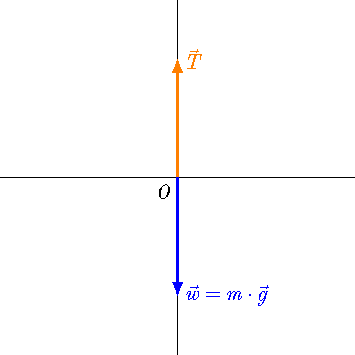
\includegraphics[height = 5cm]{IMAGENES/REFLEXIÓN/tikz.pdf}
	\caption{Representación de 1--3.}
\end{minipage}\hspace{5mm}
\begin{minipage}{0.5\linewidth}
	\centering
	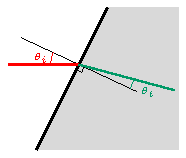
\includegraphics[height = 5.5cm]{IMAGENES/TRANSMISION/tikz.pdf}
	\caption{Representación de 4--6.}
\end{minipage}
\end{figure}\\
Se tiene conocimiento de dos modelos fenomenológicos acerca del objeto que constituye la luz. La \textit{teoría corpuscular}, que argumenta la existencia de una partícula llamada fotón, que viaja e interactúa con el resto de materia. Y la \textit{teoría electromagnética}, que consiste en tratar a la luz como una función de onda  de radiación, generada por el campo magnético y eléctrico. Ambas visiones comparten el mismo conjunto de características axiomáticas (1--6) acerca de la luz.
% )))

\subsubsection{Ley de Reflexión.} % (((
\label{subs:ley_de_refraccion}
Se ha definido el \textbf{ángulo de incidencia \(\theta _i\)}, como el ángulo agudo generado por la normal con el rayo incidente. Y se define de manera análoga el \textbf{ángulo de reflexión \(\theta _r\)}, como lo indica la Figura 1. Cuando el medio en que se propaga la luz es \textit{transparente}, y la superficie impactada es plana y \textit{reflejante}, se considerarán implíctamente las propiedades de movimiento (1--3). Así, la propiedad \ref{enu:ley_reflexion}, se escribe de la siguiente manera.
\begin{equation}
	\theta _i = \theta _r
	\label{eq:ley_reflexion}
\end{equation}
Y se llama la \textbf{Ley de Reflexión}. Veáse \([\)\cite{fisica_1}\(]\) para el desarrollo y construcción de estas definiciones en superficies planas.
% )))

\subsubsection{Ley de Snell.} % (((
\label{subs:ley_de_snell}
Se define el \textbf{ángulo de transmisión \(\theta _t\)} como el ángulo agudo que generan las semirectas del rayo transmitido, con la normal a la superficie, como lo muestra la Figura 2. La transmisión de luz ocurre cuando los dos medios de propagación son \textit{transparentes}.
\begin{figure}[ht]
	\centering
	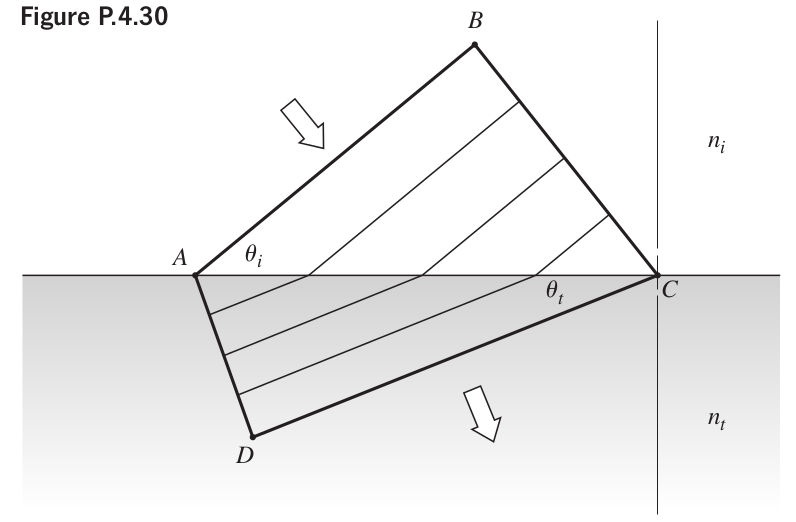
\includegraphics[width= 0.7 \linewidth]{IMAGENES/snell.png}
	\caption{Refracción de frentes de onda en una superficie plana.}
	\label{fig:snell}
\end{figure}\\
Notar que \(\theta _i\) en la Figura \ref{fig:snell}, es el ángulo de incidencia, puesto que el triángulo formado con la normal es semejante al triángulo \(ABC\). Análogamente se tiene el mismo análisis para \(\theta _t\). \\[2mm]
Se asume, que entra el mismo número de frentes de onda a la superficie, que los que se transmiten en ella, así como lo indica la Figura \ref{fig:snell}. (Tomada de \([\)\cite{fisica_1}\(]\)). Es decir,
\[
	\dfrac{\sin \theta _i}{BC} = \dfrac{\sin \theta _t}{AD}.
\]
En particular, que \(\dfrac{AD}{BC} = \dfrac{\sin \theta _t}{\sin \theta _i}\), cumpliéndose la propiedad 6. Se define la \textbf{velocidad de la luz en el medio \(A\)}, como \(v_A= \dfrac{\mbox{longitud en que pasa 1 frene de onda en }A}{\Delta t}\), donde \(\Delta t\), es el tiempo en que la luz recorre un frente de onda. Así, \(v_i = \dfrac{BC}{\Delta t}\), y \(v_t = \dfrac{AD}{\Delta t}\). De la ecuación anterior se obtiene,
\[
	\dfrac{\sin \theta _i}{v_i} = \dfrac{\sin \theta _t}{v_t}.
\]
Finalmente, se define el \textbf{índice de refracción del medio \(A\)} como \(n_A = c/v_A\). Es decir, se tiene \(n_i=c/v_i\), y \(n_t=c/v_t\). Y como consecuencia,
\begin{equation}
	n_i \sin \theta _i = n_t \sin \theta _t.
	\label{eq:snell}
\end{equation}
La ecuación (\ref{eq:snell}) se llama \textbf{Ley de Snell}. Veáse \([\)\cite{fisica_1}\(]\), para el análisis de las propiedades (1--6).
% )))

\subsubsection{Concatenación de la Ley de Snell.} % (((
\label{subs:concatenacion}
Analicemos en caso en que un mismo rayo atraviese distintas superficies.
\begin{figure}[ht]
\begin{minipage}{0.3\linewidth}
	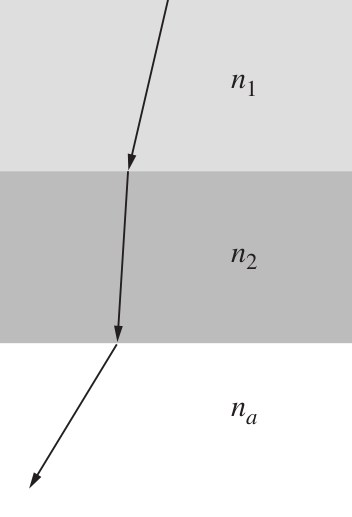
\includegraphics[width= 0.9 \linewidth]{IMAGENES/concatenacion.png}
	\caption{Múltiple Ley de Snell.}
	\label{fig:concatenacion}
\end{minipage}
\hspace{5mm}
\begin{minipage}{0.7\linewidth}
\addfontfeature{LetterSpace=-5}
	Supóngase que se tienen \(k\) medios distintos de supeficies planas paralelas entre sí, con índices de refracción \(n_1, \;\ldots,\; n_k\), así como lo indica la Figura \ref{fig:concatenacion}. Por la Ley de Snell, de la ecuación (\ref{eq:snell}) tenemos
	\begin{equation}
		\begin{array}{rcl}
			n_1 \sin \theta _1 & = & n_2 \sin \theta _2 \\[2mm]
			& = & n_3 \sin \theta _3 \\[2mm]
			& \vdots & \\[2mm]
			& = & n_k \sin \theta _k .
		\end{array}
		\label{eq:multiple_snell}
	\end{equation}
	Indicando que, para considerar el ángulo de transmisión resultante, basta con apilcar la ecuación (\ref{eq:snell}) al primer y último medio en que se transmite el haz de luz.
\end{minipage}
\end{figure}
% )))

% )))

\newpage

\subsection{--- Métodos de Análisis Experimental ---} % (((
Se realizaron dos procedimientos experimentales distintos.

\subsubsection{Reflexión en un Espejo Plano.} % (((
\label{subs:reflexion_espejo}
Se desea comprobar la Ley de Reflexión (propiedad \ref{enu:ley_coplanares}) en una superficie reflejante planar.
Para poder verificar la ecuación (\ref{eq:ley_reflexion}), se proyectó un sólo rayo de luz, a distintos ángulos sobre una misma superficie plana que reflejó cada uno de los rayos. 
Y se realizó la rotación de la superficie plana encima de un disco graduado para la medición de tales ángulos.
Se espera obtener la función identidad, es decir, que para \(\theta _i\) seleccionado, se obtenga \(\theta _r \approx \theta _i\).
% )))

\subsubsection{Ley de Refracción.} % (((
\label{subs:ley_refraccion}
Se desea describir el comportamiento de la transmisión de un haz de luz cuando cambia de medio, y que concuerde con las características descritas (1--6). Más aún, se desea comprobar la Ley de Snell (propiedad \ref{enu:snell_2}), y obtener numéricamente el índice de refracción del medio transmitido (agua).
Para poder verificar la ecuación (\ref{eq:snell}), se proyectó un único haz de luz, a distintos ángulos de incidencia, en contra de una misma superficie plana de plástico transparente, que contiene agua en su interior, que transmitió el rayo de luz a su ángulo correspondiente.
Nuevamente, se rotó la superficie y el nuevo medio de transmisión sobre un disco giratorio con graduación de los ángulos para obtener la medición experimental de los ángulos de incidencia, reflexión, y transmisión.
Con los datos de ambos ángulos \(\theta _i\) y \(\theta _t\), y tomando el índice de refracción del aire \(n_i=1\), se espera obtener \(n_t \approx 1.33\), que es el dato publicado en \([\)\cite{resnick}\(]\).
% )))

% )))

\subsection{--- Método de Mínimos Cuadrados ---} % (((
Sean \((x_i, y_i)\), con \(i=1, \;\ldots,\; n\), un conjunto de \(n\) puntos distintos. Se desea encontrar la recta \(f(x) =ax+b\), que minimice la suma de los cuadrados del error \(E(a,b) = \dis\suma_{i=1} ^n \big(ax_i+b -y_i\big) ^2\). Para ello, se obtiene el sistema lineal de las ecuaciones diferenciales \(\dfrac{\partial E}{\partial a} =0\), y \(\dfrac{\partial E}{\partial b} =0\). Cuyas soluciones son las siguientes.
\begin{equation}
	\begin{array}{rcl}
		a&=&\dfrac{n\left(\dis\suma_{i=1}^n x_i y_i\right)-\left(\dis\suma_{i=1}^n x_i \right)\left(\dis\suma_{i=1}^n y_i\right) }{n \left(\dis\suma_{i=1}^n x_i^2\right)-\left(\dis\suma_{i=1}^n x_i\right)^2} \\[1.6cm]
		b&=&\dfrac{\left(\dis\suma_{i=1}^n x_i^2\right)\left(\dis\suma_{i=1}^n y_i\right)-\left(\dis\suma_{i=1}^n x_i \right)\left(\dis\suma_{i=1}^n x_i y_i\right) }{n \left(\dis\suma_{i=1}^n x_i^2\right)-\left(\dis\suma_{i=1}^n x_i\right)^2}
	\end{array}
	\label{eq:intercept}
\end{equation}
Consúltese \([\)\cite{mont}\(]\), para la resolución del sistema lineal.
% )))

% )))

\newpage

\section{METODOLOGÍA.} % (((
La incertidumbre del único instrumento de medición empleado en la práctica (disco graduado) es de $\Delta \theta=\pm 0.5^{\circ}$.
\subsection{--- Ley de Reflexión ---} % (((
\label{sub:ley_refl_metodo}
La Figura \ref{fig:dispositivo} muestra la configuración para el dispositivo experimental usado.  Se enciende la lampara de tal manera que, al tener contacto con el material reflejante, este funciona como espejo reflejando la luz la cual se puede medir su ángulo de refracción mediante el disco graduado.
\begin{figure}[ht]
	\centering
	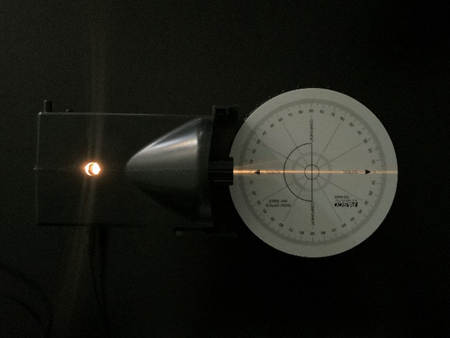
\includegraphics[width= 0.4 \linewidth]{IMAGENES/METODOLOGÍA/image_1}
	\caption{Lámpara alineada al disco graduado giratorio.}
	\label{fig:dispositivo}
\end{figure}\\
Dado que se requiere conocer el ángulo de reflexión del haz de luz generado por el espejo se procede a alinearlo para que la lámpara y el disco graduado produzcan inicialmente un ángulo de incidencia de 0°, para ello dado que el espejo tiene en su base una forma plana, este se posiciona en la marca indicada del disco graduado. \\[2mm]
Al tener calibrado el dispositivo experimental se procede a girar, sin tocar el espejo, al disco de tal forma que por un lado observamos el ángulo de incidencia y por el otro el ángulo de reflexión como se muestra en la Figura \ref{fig:foto_reflexion}.\\[-3mm]
\begin{figure}[ht]
	\centering
	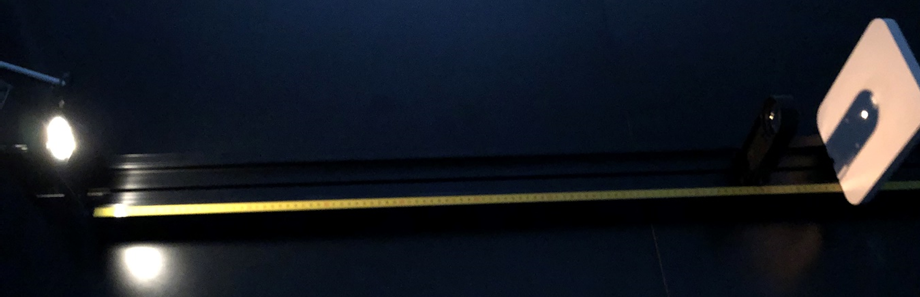
\includegraphics[width= 0.4 \linewidth]{IMAGENES/METODOLOGÍA/image_2}
	\caption{Visualización de la reflexión del haz de luz generado por la lámpara y el espejo (cara del objeto) donde se muestra el ángulo de incidencia y de reflexión.}
	\label{fig:foto_reflexion}
\end{figure}
\newpage
De esta manera, para 7 ángulos distintos positivos menores a \(90^ \circ\) se registró el ángulo de reflexión correspondiente para poder compararlos entre sí.
% )))

\subsection{--- Ley de Snell ---} % (((
\label{sub:ley_snell_metodo}
Ahora, con la misma configuración para el dispositivo experimental usado cambiamos el material por un recipiente con agua, así pues, se enciende la lampara de tal manera que, al tener contacto con el recipiente con agua, este funciona como espejo reflejando parte de la luz la cual se puede medir su ángulo de reflexión mediante el disco graduado a su vez que la otra parte genera un ángulo de refracción dentro del agua. \\[2mm]
Dado que se requiere conocer tanto el ángulo de reflexión como el ángulo de refracción del haz de luz generado por la lámpara y el recipiente con agua se procede a alinearlo para que la lámpara y el disco graduado produzcan inicialmente un ángulo de incidencia de \(0^ \circ\), para ello dado que el recipiente tiene también en su base una forma plana, este se posiciona en la marca indicada del disco graduado. \\[2mm]
Al tener calibrado el dispositivo experimental se procede a girar, sin tocar el recipiente, al disco de tal forma que por un lado observamos el ángulo de incidencia y el ángulo de reflexión y por el otro el ángulo de refracción como se muestra en las Figuras \ref{fig:rayo} y \ref{fig:flash}.
\begin{figure}[ht]
	\begin{minipage}{0.45\linewidth}
		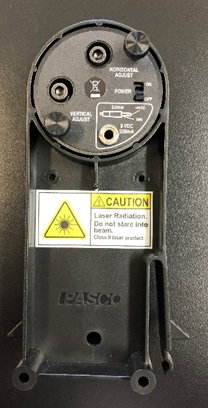
\includegraphics[width= 0.9 \linewidth]{IMAGENES/METODOLOGÍA/image_3}
		\caption{Visualización de la reflexión y refracción del haz generado por la lámpara y el recipiente con agua donde se muestra el ángulo de incidencia, de reflexión y de refracción.}
		\label{fig:rayo}
	\end{minipage}\hspace{5mm}
	\begin{minipage}{0.45\linewidth}
		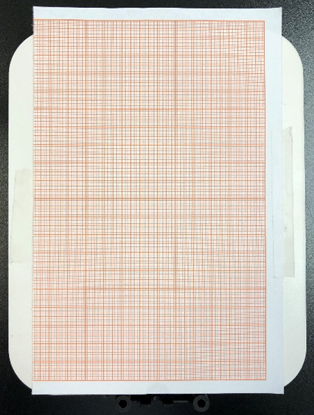
\includegraphics[width= 0.9 \linewidth]{IMAGENES/METODOLOGÍA/image_4}
		\caption{Situación de la Figura 7, tomada con flash para poder visualizar el recipiente. Se marca para resaltar, con flechas azules, lo respectivo a incidencia, reflexión y refracción.}
		\label{fig:flash}
	\end{minipage}
\end{figure}\\
De esta manera, para 7 ángulos distintos positivos menores a \(90^ \circ\) incluyendo el ángulo de \(0 ^ \circ\), se registró el ángulo de reflexión y el de refracción correspondientes para poder compararlos. \\[2mm]
% )))

% )))

\section{RESULTADOS.} % (((

\subsection{--- Ley de Reflexión ---} % (((
\label{sub:ley_reflexion_resul}
Para el primer experimento se realizaron las mediciones correspondientes al ángulo de reflexión $\theta_r$ conforme se modificaba el ángulo de incidencia $\theta_i$ por parte del haz de luz. En la Tabla \ref{tab:exp1} se muestran los resultados obtenidos durante tal experimento para las 7 mediciones correspondientes. Ambas incertidumbres corresponden a la medición directa de tales valores.
\vspace{-8mm}
\begin{table}[ht]
	\footnotesize 
	\centering
	\caption{Variación en el ángulo de reflexión $\theta_r$ respecto al ángulo de incidencia $\theta_i$.}
	\begin{tabular}{cc}
		\hline
		Ángulo de incidencia $\theta_i \pm 0.5^{\circ}$ & Ángulo de refracción $\theta_r \pm 0.5^{\circ}$ \\\hline
		\(10^ \circ \) & \(10^ \circ \) \\ \hline 
		\(20^ \circ \) & \(20^ \circ \) \\ \hline 
		\(30^ \circ \) & \(30^ \circ \) \\ \hline 
		\(40^ \circ \) & \(40^ \circ \) \\ \hline 
		\(50^ \circ \) & \(50^ \circ \) \\ \hline 
		\(60^ \circ \) & \(60^ \circ \) \\ \hline 
	\end{tabular}
	\label{tab:exp1}
\end{table}\\[-3mm]
Aplicando el método de mínimos cuadrados (el cálculo se remite a la sección \ref{sub:minimos_cuadrados}), se obtuvo que la ecuación de la recta que interpola los datos está dada por: \vspace{-2mm}
$$\theta_r=(1)\theta_i\vspace{-3mm}$$
su respectivo análisis dimensional está en la sección \ref{sub:analisis_dim_reflexion}. Ahora, interpolando para algunos valores:
\begin{itemize}[noitemsep]
	\item[$\bullet$] Si $\theta_i=35^{\circ}\Longrightarrow\theta_r=35^{\circ}$
	\item[$\bullet$] Si $\theta_i=42^{\circ}\Longrightarrow\theta_r=42^{\circ}$
	\item[$\bullet$] Si $\theta_i=87^{\circ}\Longrightarrow\theta_r=87^{\circ}$
		\vspace{-2mm}
\end{itemize}
Se grafican los puntos experimentales, junto con la recta de estimación en la Figura \ref{fig:identidad}.
\begin{figure}[ht]
	\centering
	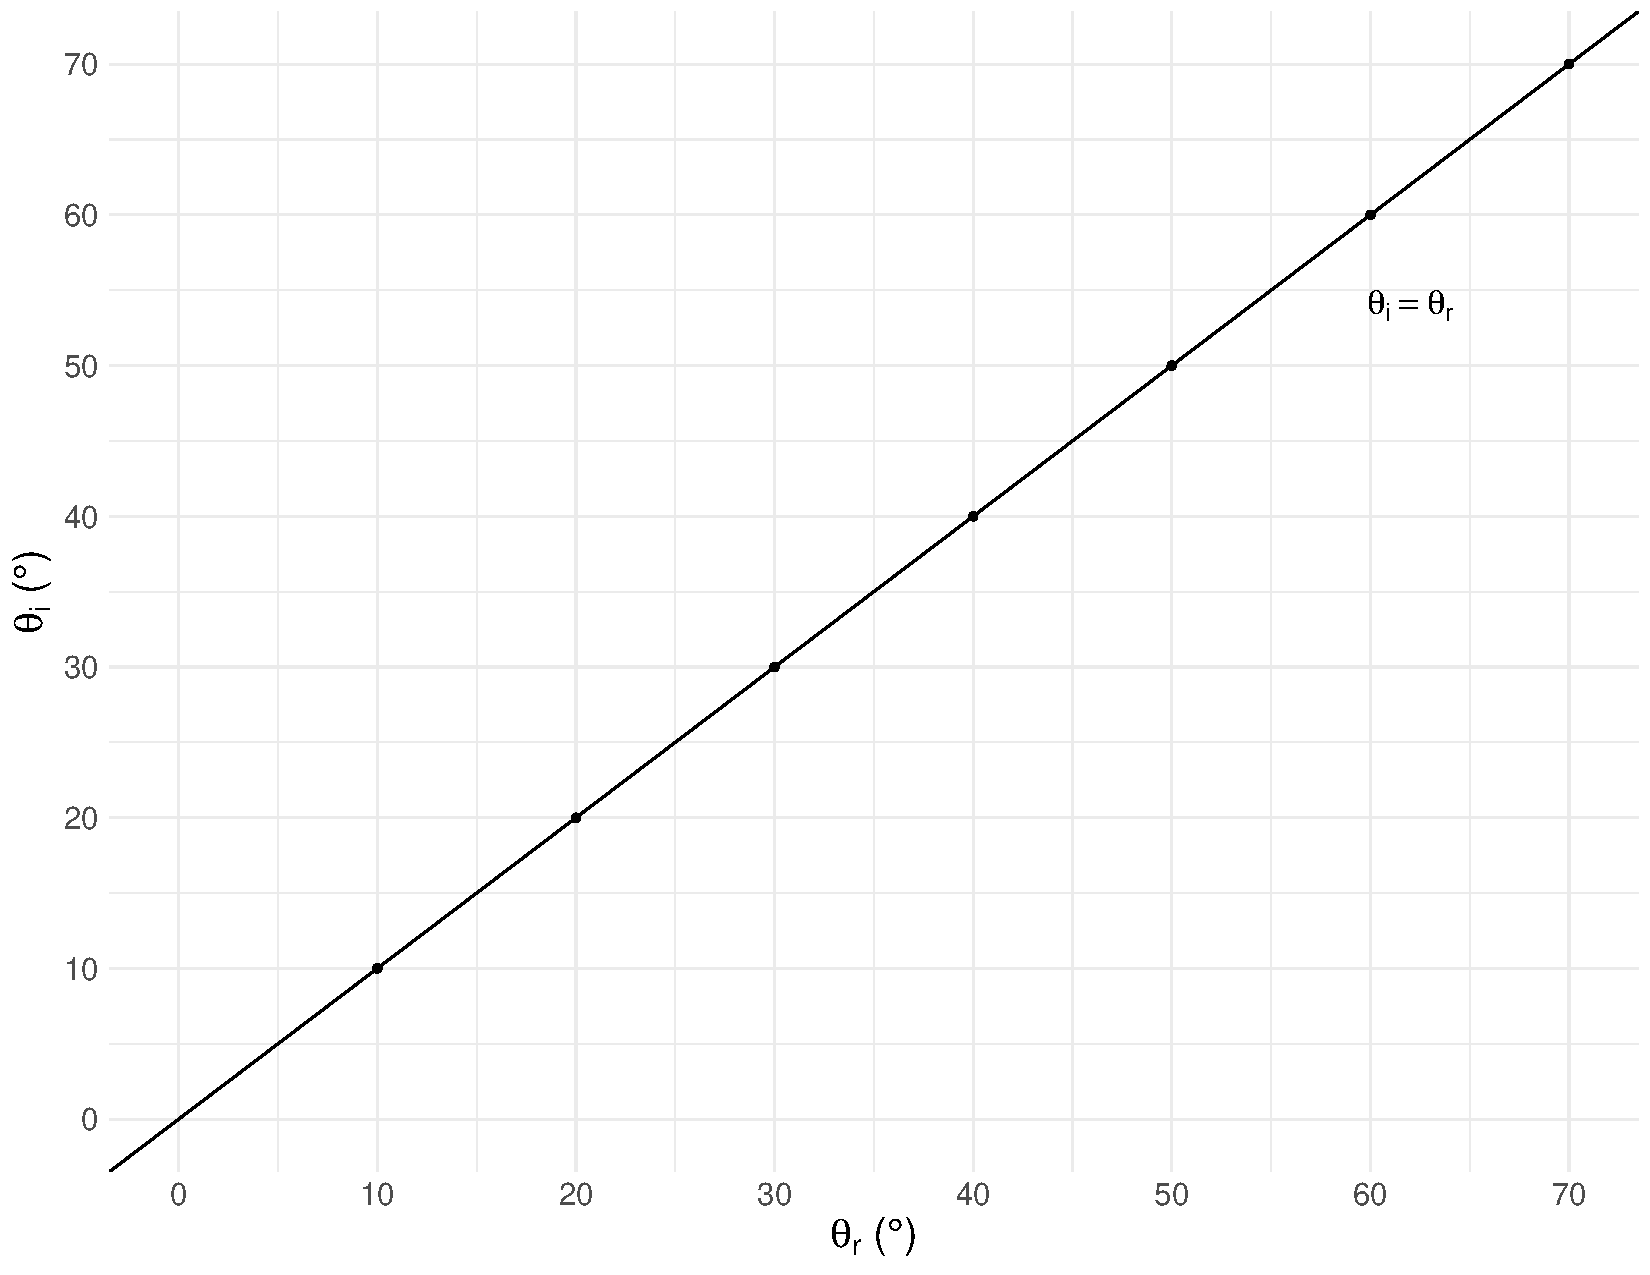
\includegraphics[width= 0.65\linewidth]{IMAGENES/ANALISIS_R/Rplot (2).pdf}
	\caption{\(\theta _i\) vs \(\theta _r\).}
	\label{fig:identidad}
\end{figure}
% )))

\subsection{--- Ley de Snell ---} % (((
\label{sub:ley_snell_resul}
En el segundo experimento se obtuvieron los ángulos de reflexión $\theta_r$ y transmisión $\theta_t$ conforme el ángulo de incidencia $\theta_i$ era modificado. Estos resultados se muestran en la Tabla 2. Ambas incetidumbres, corresponden a sus medición experimental.
\begin{table}[ht]
	\centering
	\caption{Variación de los ángulos de reflexión $\theta_r$ y transmisión $\theta_t$ respecto al ángulo de incidencia $\theta_i$.}
	\begin{tabular}{*{3}{l}}
		\hline
		$\theta_i\pm0.5^{\circ}$ & $\theta_r\pm0.5^{\circ}$ & $\theta_t\pm0.5^{\circ}$ \\ \hline 
     \(0^ \circ \)  & \(0^ \circ \)    &  \(0^ \circ \) \\ \hline 
		\(10^ \circ \) & \(10^ \circ \)   & \(7.5^ \circ \) \\ \hline 
		\(20^ \circ \) & \(20^ \circ \)   &  \(15^ \circ \) \\ \hline 
		\(30^ \circ \) & \(30^ \circ \)   &\(21.5^ \circ \) \\ \hline 
		\(40^ \circ \) & \(41^ \circ \)   &  \(29^ \circ \) \\ \hline 
		\(50^ \circ \) & \(50.5^ \circ \) &  \(35^ \circ \) \\ \hline 
		\(60^ \circ \) & \(61^ \circ \)   &  \(41^ \circ \) \\ \hline 
	\end{tabular}
	\label{tab:exp2}
\end{table}\\
A continuación se calculó el seno correspondiente a $\theta_t$ y $\theta_i$. Sus incertidumbres son colocadas en la sección \ref{sub:incert_snell}.
\begin{table}[ht]
	\centering
	\caption{Resultados de calcular $\sin(\theta_t)$ y $\sin(\theta_i)$ con las mediciones anteriores.}
	\begin{tabular}{ccc}
		\hline
		$\sin(\theta_t\pm\Delta\theta_t)$ && $\sin(\theta_i\pm\Delta\theta_i)$ \\
		\hline
		$0\pm0.0087$ && $0\pm0.0087$ \\
		\hline
		$0.1305\pm0.0086$ && $0.1736\pm0.0085$ \\
		\hline
		$0.2588\pm0.0084$ && $0.3420\pm0.0082$ \\
		\hline
		$0.3665\pm0.0081$ && $0.5000\pm0.0075$ \\
		\hline
		$0.4848\pm0.0076$ && $0.6427\pm0.0066$ \\
		\hline
		$0.5735\pm0.0071$ && $0.7660\pm0.0056$ \\
		\hline
		$0.6560\pm0.0065$ && $0.8660\pm0.0043$ \\
		\hline
	\end{tabular}
	\label{tab:senos}
\end{table}\\
Después de haber aplicado el método de mínimos cuadrados para describir el $\sin(\theta_i)$ en función de $\sin(\theta_t)$, (el código se remite nuevamente a la sección \ref{sub:minimos_cuadrados}), se obtuvo que
\begin{equation}
	\sin(\theta_i)=(1.3265 \pm 0.0111)\sin(\theta_t)+(0.0019 \pm 0.0046)
	\label{eq:ultima_ley_snell}
\end{equation}
(El análisis dimensional se remite a la sección \ref{sub:analisis_dim_snell}). Se reporta el índice de refracción del medio transmitido (agua) de:
\begin{equation}
	n_2 = 1.3265 \pm 0.0111
	\label{eq:indice_agua}
\end{equation}
Se colocan los datos experimentales, junto con la recta de regresión estimada en la Figura \ref{fig:comprobacion}.
\newpage
\begin{figure}[ht]
	\centering
	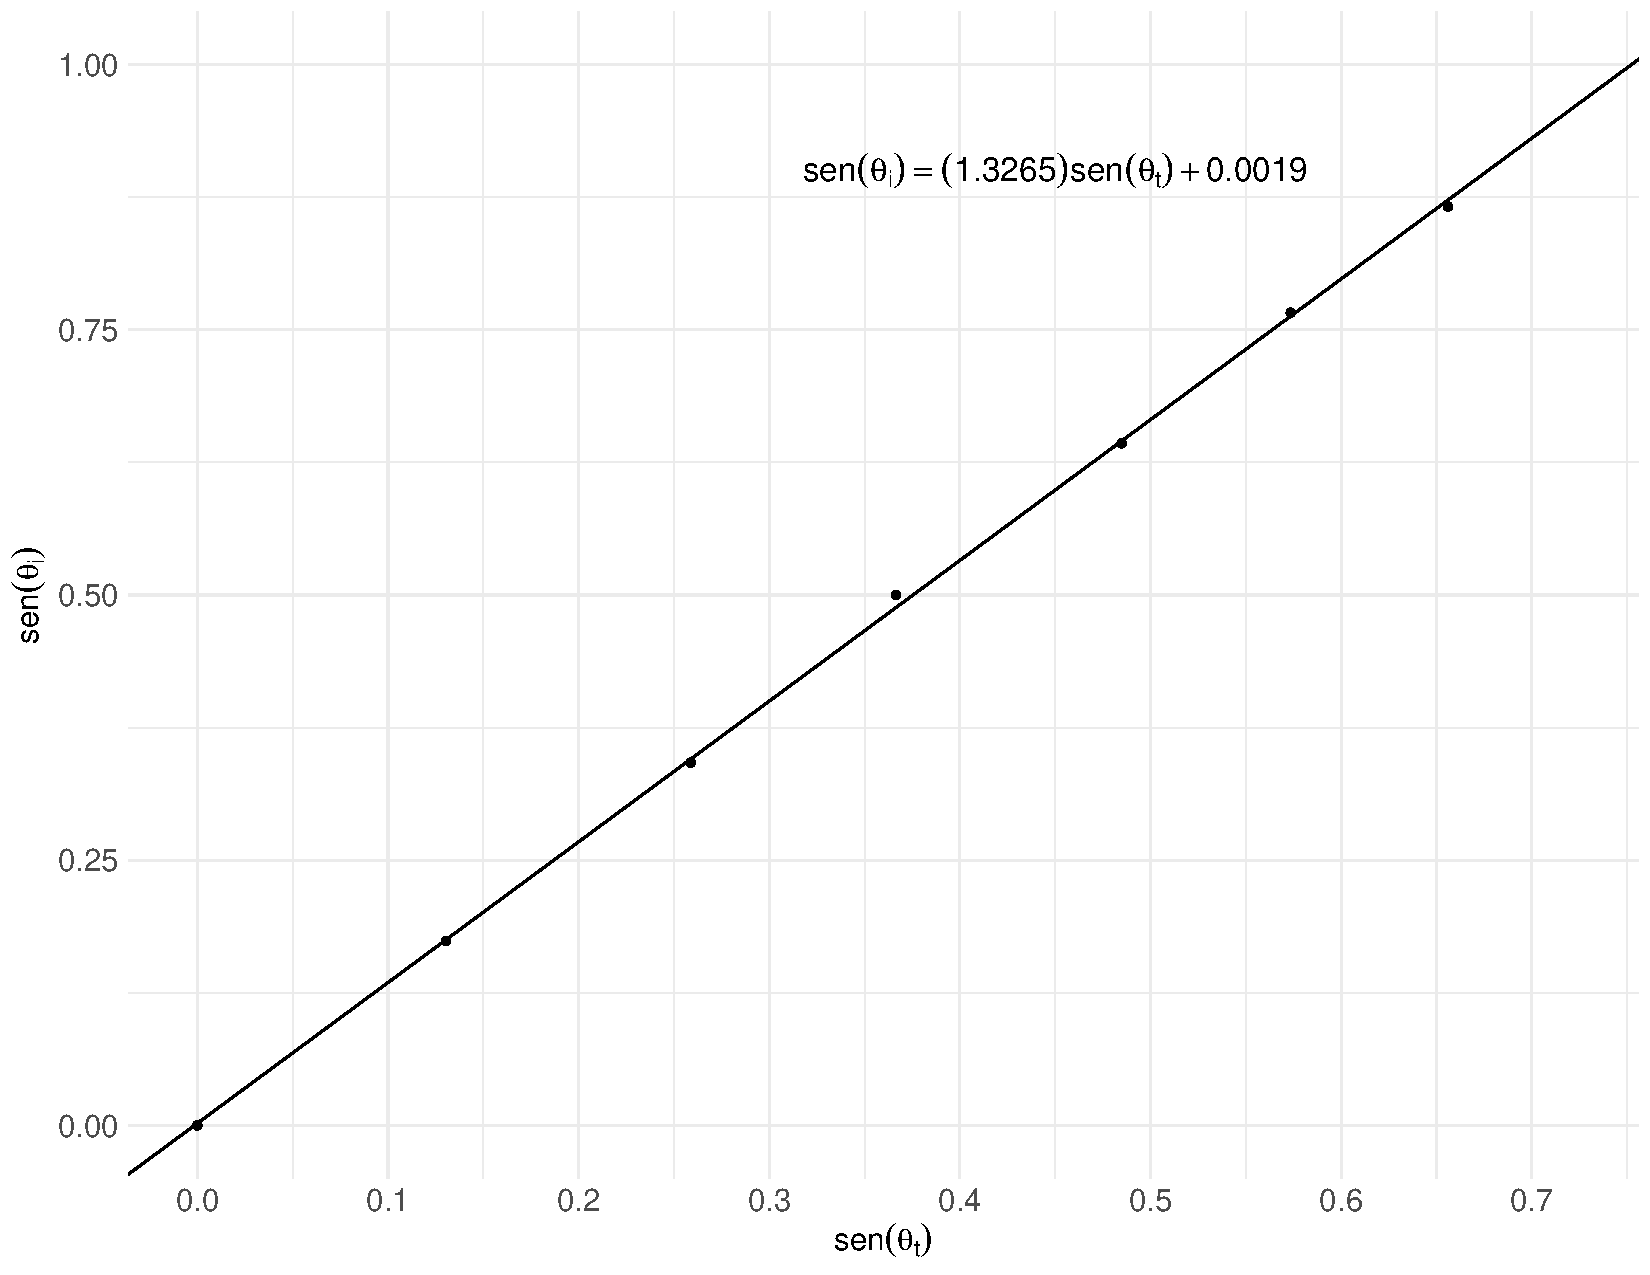
\includegraphics[width= 0.9 \linewidth]{IMAGENES/ANALISIS_R/Rplot.pdf}
	\caption{Recta de Regresión estimada de \(\sin \theta _t = a \sin \theta _i+b\).}
	\label{fig:comprobacion}
\end{figure}
% )))

% )))

\section{DISCUSIÓN DE RESULTADOS Y CONCLUSIONES.} % (((

\subsection{--- Ley de Reflexión ---} % (((
\label{sub:ley_reflexion_conc}
Para el primer experimento, cuando se giraba el material reflejante, en el cual el haz de luz  incidía sobre este, se pudo observar claramente que el reflejo del haz en el espejo tenía exactamente el mismo ángulo que el del haz incidente, por lo que con las condiciones que se tenían en este experimento (la superficie lisa del espejo y la apropiada iluminación en el laboratorio) se comprobó adecuadamente la ley de reflexión. Además, con la estimación de la recta de mínimos cuadrados se verificó el hecho enunciado en esta ley, la pendiente muestra que la razón de cambio entre el ángulo $\theta_i$ y $\theta_r$ es igual a 1, por lo que si uno aumenta (o disminuye) en cierta cantidad, el otro también lo hará exactamente en la misma proporción, además, como el valor de la ordenada al origen es cero, esto nos dice que cuando el ángulo de incidencia es normal a la superficie, el ángulo de reflexión también lo es. Así, puesto que la estimación resultó en la función identidad, se puede concluir entonces que el ángulo de incidencia $\theta_i$ era igual al ángulo de reflexión $\theta_r$ en este experimento. \\[2mm]
Con esto se verificó experimentalmente la Ley de Reflexión con una superficie plana, y un haz de luz a distintos ángulos de incidencia dados, rotando la superficie.
% )))

\subsection{--- Ley de Snell ---} % (((
\label{sub:ley_snell_conc}
Por otro lado, cuando se realizó el segundo experimento en donde se medía tanto el ángulo de reflexión $\theta_r$ como el de transmisión $\theta_t$, conforme se iba modificando el ángulo de incidencia $\theta_i$ se observaba como el haz refractado en el recipiente con agua era desviado, por lo que el valor de $\theta_t$ difería de los otros dos ángulos; el ángulo de reflexión no coincidió en tres observaciones (como se observa en la Tabla \ref{tab:senos}) con el ángulo de incidencia, pero esto se debía a que conforme aumentaba el ángulo $\theta_i$ el haz de luz reflejado se volvía cada vez más tenue, dificultando la medición de $\theta_r$, para futuras experimentaciones se recomienda una lámpara más potente y un ambiente con menos iluminación. Ya con las mediciones de los ángulos, se obtuvieron los valores correspondientes al seno de $\theta_i$ y $\theta_t$ y con estos se estimó la ecuación de la recta. El valor de la pendiente corresponde al índice de refracción del agua obtenido con respecto al índice de refracción del aire, y la justificación de este hecho se encuentra en el apéndice. Se obtuvo que tal índice de refracción en el agua era de $1.3265\pm 0.0111$, mientras que en \([\)\cite{resnick}\(]\) es $1.33\in \left(1.3154 ,1.3376\right)$, por lo que el valor experimental obtenido tiene solo un $0.26$\textsc{\%} de error con respecto al valor publicado. Por otro lado, el valor de la ordenada al origen fue de $0.0019\pm 0.0046$, lo que dice que cuando el ángulo de incidencia es normal a la superficie ($\theta_i=0^{\circ}$), el ángulo de refracción será de $\mbox{arcsen}(0.0019\pm 0.0046)=(0.1\pm0.0045)^{\circ}$.  \\[2mm]
Ahora, para la influencia del recipiente de plástico, dado que el haz de luz no interactuaba directamente con el agua al tener que pasar  por él, y por lo visto en la sección 2.1.4., el ángulo de refracción final (en este caso en el agua) no se ve afectado por la cantidad de medios que atraviesa el haz de luz, pero sí la posición del haz al tenerse una traslación del punto de contacto con la superficie, lo que implica que el valor que se midió no era el real, es decir, no corresponde con el ángulo de transmisión de la interacción del haz de luz directamente con el agua. Pero,  ya que no se conoce el grosor del plástico, no era posible dar una incertidumbre numérica que genere al final el grado de refracción del haz de luz, y dado que éste era menor a 2.5mm, se optó por despreciarlo. \\[2mm]
Entonces, se comprobó de forma experimental la Ley de Snell en la ecuación (\ref{eq:ultima_ley_snell}), mediante la medición de ángulos de incidencia, reflexión y refracción del haz de luz, rotando la superficie en un disco graduado.
% )))

% )))

% === REFERENCIAS === (((
\bibliography{Referencias}
\bibliographystyle{unsrt}
% )))

\section{APÉNDICE.} % (((

\subsection{--- Incertidumbres de la Sección \ref{sub:ley_snell_resul} ---} % (((
\label{sub:incert_snell}
Consúltese \([\)\cite{incert}\(]\), para la deducción de la ecuación (\ref{eq:incert}). Si $f$ es una función de $\mathds{R}^n$ a $\mathds{R}$ en la cual se le pueden medir sus variables (cada una asociada con su respectiva incertidumbre)
$$f(x_1\pm\Delta x_1, \;\ldots,\; x_n \pm \Delta x_n)$$
entonces (si la función es derivable) la propagación de la incertidumbre está dada por 
\begin{equation}
	\Delta f=\displaystyle\suma_{i=1}^n\Delta x_i\cdot\left|\dfrac{\partial f(x_i)}{\partial x_i}\right|
	\label{eq:incert}
\end{equation}
En este caso, se tiene, sustituyendo en la ecuación (\ref{eq:incert})
\begin{equation}
	\begin{array}{rcl}
		\sin (\theta \pm \Delta \theta) & = & f(x\pm \Delta x) \\[2mm]
		& = & f(x) \pm \Delta f \\[2mm]
		& = & \sin (\theta) \pm \Delta \theta \cdot \left| \dfrac{d \sin \theta}{d \theta} \right| \\[5mm]
		& = & \sin (\theta) \pm \Delta \theta \cdot \big| \cos \theta \big| .
	\end{array}
	\label{eq:incert_2}
\end{equation}
Realizando los cálculos, con respecto a la ecuación (\ref{eq:incert_2}), para el ángulo de transmisión $\theta_t$:
\begin{align*}
	\footnotesize
	\sin(0^{\circ}\pm0.5^{\circ})&    = \sin(0^{\circ})\pm(0.5^{\circ})\cdot\left(\dfrac{2\pi}{360^{\circ}}\right)\cdot|1|            = 0\pm0.0087\\[2mm]
	\sin(7.5^{\circ}\pm0.5^{\circ})&  = \sin(7.5^{\circ})\pm(0.5^{\circ})\cdot\left(\dfrac{2\pi}{360^{\circ}}\right)\cdot|0.9914|  = 0.1305\pm0.0086\\[2mm]
	\sin(15^{\circ}\pm0.5^{\circ})&   = \sin(15^{\circ})\pm(0.5^{\circ})\cdot\left(\dfrac{2\pi}{360^{\circ}}\right)\cdot|0.9659|  = 0.2588\pm0.0084\\[2mm]
	\sin(21.5^{\circ}\pm0.5^{\circ})& = \sin(21.5^{\circ})\pm(0.5^{\circ})\cdot\left(\dfrac{2\pi}{360^{\circ}}\right)\cdot|0.9304|  = 0.3665\pm0.0081\\[2mm]
	\sin(29^{\circ}\pm0.5^{\circ})&   = \sin(29^{\circ})\pm(0.5^{\circ})\cdot\left(\dfrac{2\pi}{360^{\circ}}\right)\cdot|0.8746|  = 0.4848\pm0.0076\\[2mm]
	\sin(35^{\circ}\pm0.5^{\circ})&   = \sin(35^{\circ})\pm(0.5^{\circ})\cdot\left(\dfrac{2\pi}{360^{\circ}}\right)\cdot|0.8191|  = 0.5735\pm0.0071\\[2mm]
	\sin(41^{\circ}\pm0.5^{\circ})&   = \sin(41^{\circ})\pm(0.5^{\circ})\cdot\left(\dfrac{2\pi}{360^{\circ}}\right)\cdot|0.7547|  = 0.6560\pm0.0065
\end{align*}
Para el ángulo de incidencia $\theta_i$
\begin{align*}
	\sin(0^{\circ}\pm0.5^{\circ})&   =\sin(0^{\circ})\pm(0.5^{\circ})\cdot\left(\dfrac{2\pi}{360^{\circ}}\right)\cdot|1|             =0\pm0.0087\\[2mm]
	\sin(10^{\circ}\pm0.5^{\circ})&  =\sin(10^{\circ})\pm(0.5^{\circ})\cdot\left(\dfrac{2\pi}{360^{\circ}}\right)\cdot|0.9848|   =0.1736\pm0.0085\\[2mm]
	\sin(20^{\circ}\pm0.5^{\circ})&  =\sin(20^{\circ})\pm(0.5^{\circ})\cdot\left(\dfrac{2\pi}{360^{\circ}}\right)\cdot|0.9396|  =0.34202\pm0.0082\\[2mm]
	\sin(30^{\circ}\pm0.5^{\circ})&  =\sin(30^{\circ})\pm(0.5^{\circ})\cdot\left(\dfrac{2\pi}{360^{\circ}}\right)\cdot|0.8660|   =0.5000\pm0.0075\\[2mm]
	\sin(40^{\circ}\pm0.5^{\circ})&  =\sin(40^{\circ})\pm(0.5^{\circ})\cdot\left(\dfrac{2\pi}{360^{\circ}}\right)\cdot|0.7660|   =0.6427\pm0.0066\\[2mm]
	\sin(50^{\circ}\pm0.5^{\circ})&  =\sin(50^{\circ})\pm(0.5^{\circ})\cdot\left(\dfrac{2\pi}{360^{\circ}}\right)\cdot|0.6427|   =0.7660\pm0.0056\\[2mm]
	\sin(60^{\circ}\pm0.5^{\circ})&  =\sin(60^{\circ})\pm(0.5^{\circ})\cdot\left(\dfrac{2\pi}{360^{\circ}}\right)\cdot|0.5000|   =0.8660\pm0.0043
\end{align*}
% )))

\subsection{--- Análisis Dimensional de la Sección \ref{sub:ley_reflexion_resul} ---} % (((
\label{sub:analisis_dim_reflexion}
Para la primer recta, el análisis dimensional de la pendiente queda\\
\begin{minipage}{0.5\linewidth}
\begin{align*}
	[a]&=\dfrac{n\displaystyle\suma_{i=1}^{n}[\theta_r][\theta_i]-\displaystyle\suma_{i=1}^{n}[\theta_r]\displaystyle\suma_{i=1}^{n}[\theta_i]}{n\displaystyle\suma_{i=1}^{n}[\theta_r]^2-\left(\displaystyle\suma_{i=1}^{n}[\theta_r]\right)^2}\\[2mm]
	&=\dfrac{[\theta]\cdot[\theta]-([\theta])([\theta])}{[\theta]^2-[\theta]^2}\\[2mm]
	&=\dfrac{[\theta]^2}{[\theta]^2}\\[2mm]
	&=1
\end{align*}
\end{minipage}\hspace{5mm}
\begin{minipage}{0.5\linewidth}
\begin{align*}
		b&=\dfrac{\left(\dis\suma_{i=1}^n [\theta_r]^2\right)\left(\dis\suma_{i=1}^n [\theta_r]\right)-\left(\dis\suma_{i=1}^n [\theta_r] \right)\left(\dis\suma_{i=1}^n [\theta_r] [\theta_r]\right) }{n \left(\dis\suma_{i=1}^n [\theta_r]^2\right)-\left(\dis\suma_{i=1}^n [\theta_r]\right)^2} \\
		&= \dfrac{[\theta] \cdot [\theta] - [\theta] \cdot [\theta]}{[\theta] ^2} \\[2mm]
		&= \dfrac{[\theta] ^2}{[\theta] ^2} \\[2mm]
		&= 1.
\end{align*}
\end{minipage}
Por lo que la pendiente y la ordenada al origen, correspondientes a este experimento, son números adimensionales.
% )))

\subsection{--- Análisis Dimensional de la Sección \ref{sub:ley_snell_resul} ---} % (((
\label{sub:analisis_dim_snell}
Para la recta correspondiente al segundo experimento, se tiene lo siguiente
\begin{align*}
	[a]&=\dfrac{n\displaystyle\suma_{i=1}^{n}[\sin(\theta_t)][\sin(\theta_i)]-\displaystyle\suma_{i=1}^{n}[\sin(\theta_t)]\displaystyle\suma_{i=1}^{n}[\sin(\theta_i)]}{n\displaystyle\suma_{i=1}^{n}[\sin(\theta_t)]^2-(\displaystyle\suma_{i=1}^{n}[\sin(\theta_t)])^2}\\[2mm]
	&=\dfrac{[\sin(\theta_t)][\sin(\theta_i)]-[\sin(\theta_t)][\sin(\theta_i)]}{[\sin(\theta_t)]^2-[\sin(\theta_t)]^2}\\[2mm]
	&=\dfrac{[\sin(\theta_t)][\sin(\theta_i)]}{[\sin(\theta_t)]^2}\\[2mm]
	&=\dfrac{[\sin(\theta_i)]}{[\sin(\theta_t)]}=1
\end{align*} 
Para la ordenada al origen:
\begin{align*}
	[b]&=\dfrac{n\displaystyle\suma_{i=1}^{n}[\sin(\theta_t)]^2\displaystyle\suma_{i=1}^{n}[\sin(\theta_i)]-\displaystyle\suma_{i=1}^{n}[\sin(\theta_t)]\displaystyle\suma_{i=1}^{n}[\sin(\theta_t)][\sin(\theta_i)]}{n\displaystyle\suma_{i=1}^{n}[\sin(\theta_t)]^2-(\displaystyle\suma_{i=1}^{n}[\sin(\theta_t)])^2}\\[2mm]
	&=\dfrac{[\sin(\theta_t)]^2[\sin(\theta_i)]-[\sin(\theta_t)][\sin(\theta_t)][\sin(\theta_i)]}{[\sin(\theta_t)]^2-[\sin(\theta_t)]^2}\\[2mm]
	&=\dfrac{[\sin(\theta_t)]^2[\sin(\theta_i)]}{[\sin(\theta_t)]^2}\\[2mm]
	&=[\sin(\theta_i)]=1
\end{align*} 
Así pues, ambos coeficientes de la recta son adimensionales. Sin embargo, la pendiente de la recta proporciona información extra que no está relacionada con las unidades de medición de los datos experimentales; recordando que el índice de refracción del medio de transmisión con respecto al de incidencia está dado por 
$$n_{ti}=\dfrac{\sin(\theta_i)}{\sin(\theta_t)}$$
(el cuál es constante por la propiedad 6) en la pendiente calculada se tiene exactamente el mismo tipo de cociente
$$\dfrac{\sin(\theta_i)}{\sin(\theta_t)}$$
por lo que el valor de la pendiente indica el índice de refracción del medio de transmisión, es decir, índice de refracción del agua.
% )))

\subsection{--- Mínimos Cuadrados de los Resultados ---} % (((
\label{sub:minimos_cuadrados}
Se realizó el siguiente script en el programa \texttt{R}.
\lstinputlisting{IMAGENES/ANALISIS_R/Cuentas.R}
% )))

% )))

\end{document}
